\chapter {Linear Algebra} 
%En bette tekst om hvad det skal bruges til (i forhold til svd eller pca)\\
Linear algebra is the study of linear equations and functions. This is done by introducing the concept of vectors and matrices. This project will introduce linear algebra through the concept of linear transformations. To define the linear transformations it is necessary to define functions.
\begin{definition}{Functions from $\mathcal{S}_1$ to $\mathcal{S}_2$}
    Let $\mathcal{S}_1$ be a subset of vectors in $\mathbb{R}^n$ and $\mathcal{S}_2$ be a subset of vectors in $\mathbb{R}^m$. Then a function $f$ from $\mathcal{S}_1$ to $\mathcal{S}_2$ written as $f$: $\mathcal{S}_1 \rightarrow \mathcal{S}_2$ assigns each vector $\textbf{v} \in \mathcal{S}_1$ to an unique vector $f(\textbf{v})\in \mathcal{S}_2$. Then $\mathcal{S}_1$ is called the domain of $f$ and $\mathcal{S}_2$ the codomain of $f$. \cite[167]{LiAl}
\end{definition}
\begin{figure} [H]
    \centering
    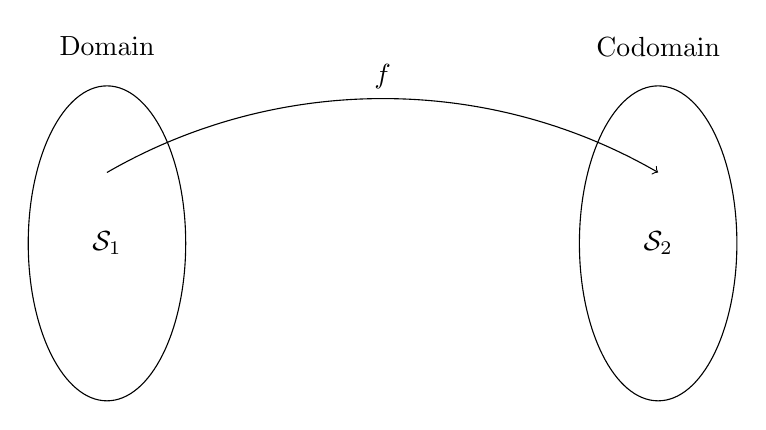
\begin{tikzpicture}
\draw(0,0)node{$\mathcal{S}_1$}circle(1 and 2);
\draw(7,0)node{$\mathcal{S}_2$}ellipse(1 and 2);
\draw [->] (0,0.9) arc (120:60:7)node[midway,anchor=south=2]{$f$};
%\draw [<-] (0,-0.9) arc (-120:-60:7)node[midway,anchor=north=2]{$f^{-1}$};
\node at (0,2.5) {Domain};
\node at (7,2.5) {Codomain};
\end{tikzpicture}
    \caption{Illustration of a function $f$: $\mathcal{S}_1 \rightarrow \mathcal{S}_2$.}
    \label{fig:s_1_to_s_2}
\end{figure}
\autoref{fig:s_1_to_s_2} illustrates a function going from $\mathcal{S}_1 \rightarrow \mathcal{S}_2$. Then a linear transformation can be defined as:
\begin{definition}{Linear Transformations}
    A function $T$: $\mathbb{R}^n \rightarrow \mathbb{R}^m$ is a linear transformation, if all $\textbf{u}, \textbf{v} \in \mathbb{R}^n$ and scalars $c \in \mathbb{R}$ satisfies that 
    \begin{align*}
        T(\textbf{u}+\textbf{v})&=T(\textbf{u})+T(\textbf{v})\\
        T(c\textbf{u})&=cT(\textbf{u}).
    \end{align*}
    \cite[171]{LiAl}
\end{definition}
A matrix vector product with a $m \times n$ matrix can be considered as a function from $\mathbb{R}^n$ to $\mathbb{R}^m$. This is called a matrix transformation and is defined as:
\begin{definition}{Matrix Transformation}
    Let $T_A(\textbf{v})=A\textbf{v}$ for an $m\times n$ matrix $A$ and $\textbf{v} \in \mathbb{R}^n$. Then the function $T_A$: $\mathbb{R}^n \rightarrow \mathbb{R}^m$ is called a matrix transformation induced by $A$. \cite[168]{LiAl}
\end{definition}
 \noindent Since a matrix vector product is linear, the matrix transformation must be too. 
\begin{theorem}{Linearity of the Matrix Transformation}
    \label{the:linearityMatrixTransformation}
    All matrix transformations are linear transformations.\cite[170]{LiAl}
\end{theorem}
\begin{proof}{Linearity of the Matrix Transformation}
     Let $T_A(\textbf{v})=A\textbf{v}$ for an $m\times n$ matrix $A$ and $\textbf{v}, \textbf{u} \in \mathbb{R}^n$. Then
     \begin{align*}
         T_A(\textbf{v}+\textbf{u})&=A(\textbf{v}+\textbf{u})=A\textbf{v}+A\textbf{u}=T_A(\textbf{u})+T_A(\textbf{v})\\
         T_A(c\textbf{v})&=A(c\textbf{v})=cA\textbf{v}=cT_A(\textbf{v}).
     \end{align*}
     From this it can be seen that all matrix transformations are linear transformations. \cite[170]{LiAl}\qedsymbol
\end{proof}

\section{Elementary Row Operations}
Linear algebra can be used to solve systems of linear equations. Below is a system with $m$ linear equations with invariables
\begin{gather*}
    a_{11}x_1+a_{12}x_2+\hdots + a_{1n}x_n = b_1\\
    a_{21}x_1+a_{22}x_2+\hdots + a_{2n}x_n = b_2\\
    \vdots \\
    a_{m1}x_1+a_{m2}x_2+\hdots + a_{mn}x_n = b_m.
\end{gather*}
This can be represented as the following matrix vector product
\begin{align*}
    \begin{bmatrix}
    a_{1 1} & a_{1 2} & \cdots & a_{1 n}\\
    a_{2 1} & a_{2 2} & \cdots & a_{2 n}\\
    \vdots  &  \vdots & \ddots & \vdots \\
    a_{m 1} & a_{m 2} & \cdots & a_{m n}\\
    \end{bmatrix}
    \begin{bmatrix}
    x_1 \\ x_2 \\ \vdots \\ x_n
    \end{bmatrix}
    = \begin{bmatrix}
    b_1 \\ b_2 \\ \vdots \\ b_m
    \end{bmatrix},
\end{align*}
and can be written as 
\begin{align*}
    A\textbf{x}=\textbf{b}
\end{align*}
where $A$ is an $m\times n$ matrix, $\textbf{x} \in \mathbb{R}^n$ and $\textbf{b} \in \mathbb{R}^m$. \cite[27-28]{LiAl}\\
To determine whether a system of linear equations has a general solution or not, there are some elementary row operations that can be done on the augmented matrix $[A\;\textbf{b}]$. The use of row operations makes it possible to reduce the augmented matrix to $[R\;\textbf{c}]$, which is an equivalent matrix. Reducing $[A\;\textbf{b}]$ to $[R\;\textbf{c}]$ makes the system of linear equations easier solved.
\begin{definition}{Elementary Row Operations}
There are three elementary row operations, that can be used to determine an equivalent system of linear equations, for a given system of linear equations.
\begin{enumerate}
    \item Interchange Operation:
    It is allowed to let two rows switch place.
    Notation: $A\xrightarrow{\textbf{r}_i\leftrightarrow \textbf{r}_t} B$ where $i$ and $t$ are rows
    \item Scaling Operation:
    Multiplying any row of a matrix with the same nonzero scalar $c$.
    Notation: $A\xrightarrow{c\textbf{r}_i\rightarrow \textbf{r}_i} B$
    \item Row Addition Operation:
    Add a multiple of one row of the matrix to another row.
    Notation: $A\xrightarrow{c\textbf{r}_i+\textbf{r}_t\rightarrow \textbf{r}_t} B$
\end{enumerate}
\cite[32]{LiAl}
\end{definition}

When replacing a given system of linear equations with one, which is easier solved, the most simple equivalent system of linear equations is called the reduced row echelon form. 
\begin{definition}{Reduced Row Echelon Form}
A matrix in row echelon form is satisfying the following three conditions.
\begin{enumerate}
    \item Each nonzero row lies above every zero row.
    \item The leading entry of a nonzero row is in a column to the right of the column containing the leading entry of any preceding row.
    \item All entries below a leading entry are $0$.
\end{enumerate}
Pivot positions are the first non zero entry of each row, the pivot columns are the columns containing the pivot positions. 
For a matrix to be in reduced echelon form it has to satisfy two conditions more. 
\begin{enumerate}
    \item For a column with a leading entry of some row, all other entries have to be 0.
    \item The leading entries has to be equal to 1.
\end{enumerate}
\cite[33]{LiAl}
\end{definition}
A system of linear equations can be whether consistent or inconsistent. For a inconsistent system there is no solutions.
Otherwise for a consistent system there is either one solution or infinitely many solutions.

A system is inconsistent if the last column of the row echelon form of the augmented matrix is a pivot column. Since this is equivalent to $0\cdot x_1+0\cdot x_2+\hdots + 0\cdot x_n=c$ where $c\neq 0$. \\
The following example shows the method of solving a system of linear equations using elementary row operations.
\begin{example}{Reduced Row Echelon Form}
Given a system of linear equations
\begin{align*}
    x_1-x_3-2x_4-8x_5&=-3\\
    -2x_1+x_3+2x_4+9x_5 &= 5\\
    3x_1-2x_3-3x_4-15x_5&=-9.
\end{align*}
To determine the general solution for the system, the first step is to calculate the row echelon form of the augmented matrix $[A\;\textbf{b}]$. This makes it possible to determine whether the system is consistent or inconsistent. Calculating the row echelon form yields
\begin{align*}
[A\;\textbf{b}] =
	&\begin{bmatrix}
	1  & 0  & -1  &-2  & -8  & -3 \\
	-2 & 0  & 1   & 2  & 9   & 5 \\
	3  & 0  & -2  & -3 & -15 & -9 
   \end{bmatrix} \\
  \xrightarrow{\substack{r_2+2r_1\rightarrow r_2\\  r_3-3r_1\rightarrow r_3}}
  &\begin{bmatrix}
 	 1 & 0 & -1 &-2  & -8 & -3 \\
 	 0 & 0 & -1 & -2 & -7 & -1 \\
	 0 & 0 & 1  & 3  & 9  & 0
  \end{bmatrix}\\
  \xrightarrow{r_3+r_2\rightarrow r_3}
    &\begin{bmatrix}
  	 \circled{1} & 0 & -1 &-2 & -8 & -3 \\
 	 0 & 0 & \circled{-1} & -2 & -7 & -1 \\
	 0 & 0 & 0 & \circled{1} & 2 & -1
       \end{bmatrix}.
\label{examplepivot}
\end{align*}
As seen in the matrix above, there are three pivot positions (circled in red), hence three pivot columns.

Since the last column of the augmented matrix not is a pivot column, the system is considered consistent. All entries in the second column is equal to zero, hence the system has infinite solutions. 
To determine the most simple equivalent system of the given linear equations, the reduced row echelon form is calculated:
\begin{align*}
  \xrightarrow{\substack{r_1+2r_3\rightarrow r_1\\r_2+2r_3\rightarrow r_2}}
    &\begin{bmatrix}
  	    1 & 0 & -1 &0 & -4 & -5 \\
 	    0 & 0 & -1 & 0 & -3 & -3 \\
	    0 & 0 & 0 & 1 & 2 & -1
     \end{bmatrix}\\
  \xrightarrow{\substack{-1r_2\rightarrow r_2}}
  &\begin{bmatrix}
  	    1 & 0 & -1 &0 & -4 & -5 \\
 	    0 & 0 & 1 & 0 & 3 & 3 \\
	    0 & 0 & 0 & 1 & 2 & -1
     \end{bmatrix}\\
     \xrightarrow{\substack{r_1+r_2\rightarrow r_1}}
     &\begin{bmatrix}
        1 & 0 & 0 & 0 &-1 &-2 \\
 	    0 & 0 & 1 & 0 & 3 & 3 \\
	    0 & 0 & 0 & 1 & 2 &-1
     \end{bmatrix}
    \end{align*}
With the reduced row echelon form, it is possible to reduce the equations to
	\begin{align*}
		x_1-x_5 =-2   &\Rightarrow x_1=x_5 -2\\
        x_3 + 3x_5 =3 &\Rightarrow x_3=-3x_5+3\\
        x_4 +2x_5 = -1 &\Rightarrow	x_4=-2x_5-1,
	\end{align*}
which can be written as
    \begin{align*}
    	\textbf{x}=
        \begin{bmatrix}
       	    x_1\\ x_2 \\ x_3\\ x_4 \\x_5
        \end{bmatrix} =
        \begin{bmatrix}
        	x_5- 2\\ x_2\\ -3x_5 +3\\-2x_5-1\\ x_5 
        \end{bmatrix}=
        \begin{bmatrix}
      	    -2\\ 0 \\ 3 \\-1 \\0
        \end{bmatrix} + x_2
        \begin{bmatrix}
            0 \\ 1 \\ 0 \\ 0 \\ 0 
        \end{bmatrix} + x_5
        \begin{bmatrix}
            1 \\ 0 \\ -3 \\ -2 \\ 1
        \end{bmatrix}.
    \end{align*}
This is the general solution for the given linear equations.
\end{example}
When a matrix is on reduced row echelon form, the number of pivot columns is called the rank, and the amount of non pivot columns is the nullity.
\begin{definition}{Rank and Nullity of a Matrix}\label{def:rank_nullity}
The rank of a $m \times n$ matrix $A$, is defined as the number of pivot columns, or the number of nonzero rows of the reduced echelon form of $A$. The rank is denoted as rank$(A)$
The nullity of $A$ is denoted as nullity$(A)$, is defined as nullity$(A)=n - $rank$(A)$.
\cite[47]{LiAl}
\end{definition}
The concepts of rank and nullity will be used in the next section where the concepts subspace and basis for $\mathbb{R}^n$, and their dimension will be introduced.
\section{Subspace, Basis and Dimension}
(intro af hvad subspace og basis bruges til, svar på spørgsmålet om hvorfor vi beskriver dette)

\begin{definition}{Linear Combination}
    A combination of vectors $\textbf{u}_1, \textbf{u}_2, \hdots, \textbf{u}_k$ is a linear combination if it is on the form
    \begin{align*}
        c_1\textbf{u}_1 + c_2\textbf{u}_2 + \hdots + c_k\textbf{u}_k
    \end{align*}
    where $c_1, c_2, \hdots, c_k$ are the scalars, which is called the coefficients of the linear combination. \cite[14]{LiAl} 
\end{definition}
A set of vectors $\mathcal{S}=\{\textbf{v}_1, \textbf{v}_2, \hdots, \textbf{v}_k\}$ is said to be linear dependent if all vectors in the set can be represented as linear combinations of the other vectors. Otherwise the vector set is linear independent.
Let $\mathcal{S}$ be linear dependent and $\textbf{v}_i$ be an arbitrary vector in $\mathcal{S}$. Then for some scalars $c_1, c_2, \hdots, c_k$
\begin{align} \label{eq:LinearIndependent}
    c_1\textbf{v}_1+c_2\textbf{v}_2+\cdots+c_k\textbf{v}_k=\textbf{v}_i,
\end{align}
which is the same as
  \begin{align*}
    c_1\textbf{v}_1+c_2\textbf{v}_2+\cdots+c_k\textbf{v}_k-\textbf{v}_i=\textbf{0}. 
 \end{align*}
 If $\mathcal{S}$ was linear independent there exists no scalars such that \eqref{eq:LinearIndependent} is true. This leads to the following definition.
\begin{definition}{Linear Dependent and Linear Independent} \label{def:LinearDependent}
    A set of vectors $\textbf{v}_1, \textbf{v}_2, \hdots, \textbf{v}_k$ is linear dependent for some scalars $c_1, c_2, \hdots, c_k$ which are not all $0$
    \begin{align*}
       c_1\textbf{v}_1+c_2\textbf{v}_2+\dots+c_k\textbf{v}_k=\textbf{0}.
    \end{align*}
    A set of vectors $\textbf{v}_1, \textbf{v}_2, \hdots, \textbf{v}_k$ is linear independent if the scalars $c_1, c_2, \hdots, c_k$, where all equals 0, such that
    \begin{align*}
        c_1\textbf{v}_1+c_2\textbf{v}_2+\dots+c_k\textbf{v}_k=\textbf{0}
    \end{align*}
    Note that, by the definitions, a set of vectors obviously is linear independent, if it is not linear dependent. \cite[75-76]{LiAl} 
\end{definition}
\noindent The vectors which is a product by a linear combination of a set of vectors is called the span of the set of vectors and is defined by:
\begin{definition} {The Span of a Set of Vectors}
A linear combinations of a nonempty set of vectors $\mathcal{S} = \{ \textbf{u}_1,\textbf{u}_2 \cdots \textbf{u}_k\}$ is denoted as $c_1 \textbf{u}_1 + c_2\textbf{u}_2+ \cdots+ c_k\textbf{u}_k$, where $\textbf{u}_1,\textbf{u}_2 \cdots \textbf{u}_k$ are in $\mathbb{R}^n$ and $c_1, c_2 \cdots c_k$ are scalars.
The span of the set of vectors is a set of all linear combinations in $\mathbb{R}^n$
\cite[66]{LiAl}
\end{definition}
An important concept in linear algebra is subspaces, which have the following properties.
\begin{definition}{Subspace}
A subspace is a set of vectors $W$ in $\mathbb{R}^n$ which have the following three properties. 
\begin{enumerate}
    \item The zero vector belongs to $W$.
    \item The sum of any vectors in the same $W$, remains in the same subspace. This means $W$ is closed under vector addition.
    \item Every scalar multiple of a vector that belongs to $W$, remains in the same $W$. This means $W$ is closed under scalar multiplication.
\end{enumerate}
\cite[227]{LiAl}
\label{exa:SubspaceDef}
\end{definition}
\noindent The following example shows how to determine whether a set of vectors is a subspace or not.
\begin{example}{Determine Whether $W$ is a Subspace or Not}
The following set of vectors is given
\begin{align*}
    W = \begin{Bmatrix}
    \begin{bmatrix}
    w_1\\w_2\\w_3\\w_4
    \end{bmatrix}
        \in \mathbb{R}^4: 2w_1 + 5w_2 - 7w_3 -2w_4 = 0 
    \end{Bmatrix}.
\end{align*}
To determine whether $W$ is a subspace or not, the three properties of Definition \ref{exa:SubspaceDef} is used. \\

\noindent 1. To determine whenever the first property from Definition \ref{exa:SubspaceDef} is satisfied, it is shown that $\textbf{0}$ is in the set.
\begin{align*}
    2(0) + 5(0) - 7(0) -2(0) = 0,
\end{align*}
hence $\textbf{0}\in W$\\
2. Having two vectors $\textbf{u}=\begin{bmatrix}
    u_1\\u_2\\u_3\\u_4\end{bmatrix}$ and $\textbf{v}=\begin{bmatrix}
    v_1\\v_2\\v_3\\v_4\end{bmatrix}$ in $W$ it must satisfy that 
    \begin{align*}
        \textbf{u}+\textbf{v} =
        \begin{bmatrix}
         u_1 + v_1 \\ u_2 + v_2 \\ u_3 + v_3 \\ u_4 + v_4
        \end{bmatrix}.  
    \end{align*}\\
    Further calculations yields
    \begin{align*}
        &\,2(u_1+v_1)+5(u_2+v_2)-7(u_3+v_3)-2(u_4+v_4)\\
        =& (2u_1+5u_2-7u_3-2u_4)+(2v_1+5v_2-7v_3-2v_4)\\ =& 0 + 0 = 0,
    \end{align*}
    hence $\textbf{u}+\textbf{v}\in W$.\\ 
3. Having a vector \textbf{u} it must satisfy 
    \begin{align*}
        c\textbf{u}=c\begin{bmatrix}
        u_1\\u_2\\u_3\\u_4\end{bmatrix}=
        \begin{bmatrix}
        cu_1\\cu_2\\cu_3\\cu_4\end{bmatrix},
    \end{align*}
    which yields
    \begin{align*}
       2(cu_1)+5(cu_2)-7(cu_3)-2(cu_4)=c(2u_1+5u_2-7u_3+2u_4)= c(0) = 0.
    \end{align*}
    As seen, when multiplying a vector in $W$, the subspace remains the same. Since all the properties of Definition \ref{exa:SubspaceDef} is satisfied $W$ is a subspace.
\end{example}
\noindent It can be shown that the span of a set of vectors in $\mathbb{R}^n$ is also a subspace of $\mathbb{R}^n$.
\begin{theorem}{Span as a Subspace of $\mathbb{R}^n$}
The span of a definite nonempty subset of $\mathbb{R}^n$ is a subspace of $\mathbb{R}^n$.
\cite[231]{LiAl}
\end{theorem}
\begin{proof}{Span as a Subspace of $\mathbb{R}^n$}
   Having a span of $\mathcal{S} = \{\mathbf{w}_1, \mathbf{w}_2, \hdots, \mathbf{w}_k$\}. It can be seen that $\mathbf{0}$ belongs to $\mathcal{S}$, by following expression:
    \begin{align*}
        0\mathbf{w}_1 + 0\mathbf{w}_2 + \hdots + 0\mathbf{w}_k = \mathbf{0}.
    \end{align*}
    If $\mathbf{u}$ and $\mathbf{v}$ belongs to $\mathcal{S}$ then
    \begin{align*}
      \mathbf{u} = a_1\mathbf{w}_1 + a_2 \mathbf{w}_2 + \hdots + a_k\mathbf{w}_k \quad \text{and} \quad \mathbf{v} = b_1\mathbf{w}_1 + b_2 \mathbf{w}_2 + \hdots + b_k\mathbf{w}_k,  
    \end{align*}
    for some scalars $a_1, a_2, \hdots, a_k$ and $b_1, b_2, \hdots, b_k$.\\ It follows that $\mathbf{u}+\mathbf{v}$ belongs to $\mathcal{S}$ since 
    \begin{align*}
     \mathbf{u}+\mathbf{v} &= (a_1\mathbf{w}_1 + a_2 \mathbf{w}_2 + \hdots + a_k\mathbf{w}_k) + (b_1\mathbf{w}_1 + b_2 \mathbf{w}_2 + \hdots + b_k\mathbf{w}_k)\\ 
     &= (a_1+b_1)\mathbf{w}_1 + (a_2+b_2)\mathbf{w}_2 + \hdots + (a_k+b_k)\mathbf{w}_k.
     \end{align*}
     Therefore $\mathcal{S}$ is closed under vector addition.\\ For any scalar $c$ it can be expressed that 
     \begin{align*}
         c\mathbf{u} &= c(a_1\mathbf{w}_1 + a_2 \mathbf{w}_2 + \hdots + a_k\mathbf{w}_k)\\
         &=(c_1a_1)\mathbf{w}_1 + (c_2a_2)\mathbf{w}_2 + \hdots + (c_ka_k)\mathbf{w}_k,
     \end{align*}
     where $c\mathbf{u}$ belongs to $\mathcal{S}$, then $\mathcal{S}$ is closed under scalar multiplication, and $\mathcal{S}$ is therefore a subspace of $\mathbb{R}^n$.\cite[231]{LiAl} \qedsymbol
\end{proof}
\noindent There are many generating sets for a nonzero subspace $V$ of $\mathbb{R}^n$, and thereby it can be convenient to determine a generating set of $V$, which contains the fewest amount of vectors as possible. The span of this generating set is called a basis.
\begin{definition}{Basis}
A basis for a nonzero subspace $V$, is a linearly independent generating set for $V$. This means that the basis contains as few vectors as possible.\cite[241]{LiAl}
\end{definition}
\noindent The following three properties are true if $\mathcal{S}$ is a finite subset of $\mathbb{R}^n$
\begin{itemize}
    \item If $\mathcal{S}$ contains at least n vectors, then $\mathcal{S}$ is a generating set for $\mathbb{R}^n$. 
    \item If $\mathcal{S}$ contains maximum n vectors then $\mathcal{S}$ is linear independent.
    \item If $\mathcal{S}$ contains precisely n vectors then $\mathcal{S}$ is a basis for $\mathbb{R}^n$.
\end{itemize}
Because a basis is a linearly independent generating set of $\mathbb{R}^n$ containing exactly $n$ vectors , there are two theorems, which provides some operations that can be done to determine a basis of the given subspace. These theorems are called Reduction theorem and Extension theorem.
\begin{theorem}{Reduction Theorem}
Having $\mathcal{S}$ as a finite generating set of a nonzero subspace $V$ of $\mathbb{R}^n$. Then by removing vectors from $\mathcal{S}$, the span can be reduced to a basis of $V$.
\cite[243]{LiAl}
\label{reductiontheorem}
\end{theorem}
Proving the \ref{reductiontheorem} the term column space of a matrix is needed. The column space of a matrix is the span of its columns. A basis for this column space is the column space only consisting of the pivot columns of $A$, since a basis must be a linearly independent generating set.
\begin{proof}{Reduction Theorem}
Having a matrix $A=\begin{bmatrix}
 \textbf{u}_1, \textbf{u}_2, \cdots, \textbf{u}_k
\end{bmatrix}$ and a span
$
\mathcal{S}=\begin{Bmatrix}
 \textbf{u}_1, \textbf{u}_2, \cdots, \textbf{u}_k
\end{Bmatrix}  
,$ which is a generating set of a nonzero subspace $V$ of $\mathbb{R}^n$. Because $\mathcal{S}$ and $A$ consist of the exact same vectors, the column space of $A$ must be a generating set of $V$. Consider the pivot columns for matrix $A$, a basis for the column space of $A$ can be determined, and is contained in $\mathcal{S}$. \qedsymbol
\end{proof}



\begin{theorem}{Extension Theorem}
Having a span $\mathcal{S}$ which is a subset of a subspace $V$, then $\mathcal{S}$ can be, by inclusion of additional vectors, extended to a basis for $V$. \cite[245]{LiAl}
\end{theorem}

\begin{proof}{Extension Theorem}
There are two cases for a linearly independent subset $\mathcal{S}$ to be extended to a basis of a nonzero subspace $V$.
First case is where the span of $\mathcal{S}$ is $V$, hence $\mathcal{S}$ is a basis of $V$.\\
Second case is where $V$ contains a vector $\textbf{v}_1$, and $\textbf{v}_1$ is not contained in a linearly independent subset $\mathcal{S}=
\begin{Bmatrix} \textbf{u}_1,\textbf{u}_2,\cdots,\textbf{u}_k \end{Bmatrix} 
 $. A possible basis for $V$ is $\mathcal{S}$ extended with $\textbf{v}_1$, if and only if $\mathcal{S'}=\begin{Bmatrix} \textbf{u}_1,\textbf{u}_2,\cdots,\textbf{u}_k, \textbf{v}_1 \end{Bmatrix}$ is linearly independent and span of $\mathcal{S'}$ is $V$. In the case that $\mathcal{S'}$ is not $V$, $\mathcal{S'}$ can be extended with another vector, denoted $\mathcal{S''}$. \qedsymbol 
\end{proof}

The Extension theorem and the Reduction theorem have given two characteristics of a basis for a subspace. These characteristics yields that vectors can be deleted and used to extend a subset and form a basis for a subspace. These characteristics result in the possibility to determine infinitely many bases for a nonzero subspace. Even though a particular subspace has infinitely many bases, the bases will always consist of the same amount of vectors, which leads to following definition.

\begin{definition}{Dimension of a Subspace}
The dimension of a nonzero subspace $V$ of $\mathbb{R}^n$ is the number of vectors in the basis. The dimension is denoted by dim $V$. The dimension of the zero subspace of $\mathbb{R}^n$ is 0 \cite[246]{LiAl}.
\end{definition}

\begin{definition}{Null space}
The solution set $A\textbf{x}=\textbf{0}$ for a matrix $A$, is the null space of the matrix. It is denoted as Null $A$. \cite[232]{LiAl}
\end{definition}

\begin{example}{Determine a Generating Set for The Null Space and the Dimension of a Matrix }
Let
\begin{align*}
    A=
    \begin{bmatrix}
    1 & 1 & -1 & 4 \\
    2 & 1 & -3 & 5\\
    -2 & 0 & 4 & -2
    \end{bmatrix}.
\end{align*}
To generate a set for Null $A$, the matrix is reduced to reduced row echelon form:

\begin{align*}
\begin{bmatrix}
    1 & 1 & -1 & 4 \\
    2 & 1 & -3 & 5\\
    -2 & 0 & 4 & -2
\end{bmatrix}\xrightarrow{\substack{r_2-2r_1\rightarrow r_2\\2r_1+r_3\rightarrow r_3}}
\begin{bmatrix}
    1 & 1 & -1 & 4 \\
    0 & -1 & -1 & -3\\
    0 & 2 & 2 & 6
\end{bmatrix}\\\xrightarrow{2r_2+r_3\rightarrow r_3}
\begin{bmatrix}
   1 & 1 & -1 & 4 \\
    0 & -1 & -1 & -3\\
    0 & 0 & 0 & 0 
\end{bmatrix}
\xrightarrow{\substack{r_1-r_2\rightarrow r_1\\(-1)r_2\rightarrow r_2}}
\begin{bmatrix}
   1 & 0 & -2 & 1 \\
    0 & 1 & 1 & 3\\
    0 & 0 & 0 & 0
\end{bmatrix},
\end{align*}
hence the general solution for $A\textbf{x}=\textbf{0}$ is
\begin{align*}
    x_1 - 2x_3 + x_4 = 0 &\Rightarrow x_1 = 2x_3 - x_4\\
    x_2 + x_3 + 3x_4 = 0 &\Rightarrow x_2=-x_3 -3x_4.
\end{align*}
Written in vector form
\begin{align*}
\begin{bmatrix}
   x_1\\x_2\\x_3\\x_4 
\end{bmatrix} =
\begin{bmatrix}
   2x_3 - x_4 \\ -x_3 -3x_4 \\ x_3 \\ x_4
\end{bmatrix} = x_3
\begin{bmatrix}
   2\\ -1\\ 1 \\0
\end{bmatrix} + x_4
\begin{bmatrix}
   -1\\ -3\\ 0\\ 1
\end{bmatrix}.
\end{align*}
The null space is then
\begin{align*}
\text{Null}\; A = 
\begin{Bmatrix}
\begin{bmatrix}
   2\\ -1\\ 1 \\0
\end{bmatrix},
\begin{bmatrix}
   -1\\ -3\\ 0\\ 1
\end{bmatrix}
\end{Bmatrix}.
\end{align*}
From this it can be seen that $\text{Null}\; A$ have dimension 2.
\end{example}

\section{Invertible Matrix}
This section introduces the concept of invertible matrices. Working with transformation of a matrix, it is often relevant to be able recreate the original matrix. This can be done using an invertible matrix, as seen on \autoref{fig:inverseFunction}, where it is possible to go from the domain to the codomain by transformation and the other way by its inverse. 
\begin{figure}[H]
    \centering
    \input{figures/Tikz/inverseFunction.tex}
    \caption{Illustration of the function $f$: $\mathcal{S}_1 \rightarrow \mathcal{S}_2$ and $f^{-1}$: $\mathcal{S}_2 \rightarrow \mathcal{S}_1$.}
    \label{fig:inverseFunction}
\end{figure}
To explain how to invert a matrix, it is defined in the following.
\begin{definition}{Invertible Matrix} \label{def:Invertible}
    An  $n \times n$ matrix $A$ is invertible, if there exists another $n \times n$ matrix $B$ which when multiplied with $A$ results in an identity matrix such as
    \begin{align*}
        AB=BA=I_n.
    \end{align*}
    In this case, $B$ can be defined as an inverse of $A$. The inverse matrix of $A$ is denoted $A^{-1}$. \cite[122]{LiAl}
\end{definition}
\noindent Not all matrices is invertible. To describe the conditions for which a matrix is invertible the concepts of an elementary matrix are introduced. This is done in \autoref{bil:ElementaryMatrix} where $P$ was defined as $P=E_K\cdots E_2E_1$, where $E$ is an elementary matrix such that:
\begin{align*}
    PA=R.
\end{align*}
For a matrix to be invertible the following theorem has to be satisfied.
\begin{theorem}{Invertible Matrix}
    \label{the:invertibleMatrix}
    If an $n \times n$ matrix $A$ is invertible, then the following statements are true:
    \begin{enumerate}
        \item The reduced row echelon form of $A$ is $I_n$
        \item $\text{rank } A = n$
        \item The equation $A\mathbf{x}=\mathbf{b}$ is consistent for every $\mathbf{b}$ in $\mathbb{R}^n$
        \item The only solution for $A\mathbf{x}=\mathbf{0}$ is $\mathbf{0}$
    \end{enumerate}
    \cite[138]{LiAl}
\end{theorem}
\begin{proof}{Invertible matrix}
\begin{enumerate}
    \item  If the reduced row echelon form of $A$ is $I_n$, there must exists an invertible $n \times n$ elementary matrix $P$ which when multiplied by $A$ is $I_n$. So
    \begin{align*}
        A=I_nA=(P^{-1}P)A=P^{-1}(PA)=P^{-1}I_n=P^{-1}.
    \end{align*}
    As seen $A=P^{-1}$, hence $A$ is invertible if the reduced row echelon form of $A$ is $I_n$. 
    \item As stated in definition \ref{def:rank_nullity} the rank of a matrix is defined as the amount of pivot columns in the reduced echelon form, and since the reduced echelon form is $I_n$ the rank will be $n$.
    \item Since the reduced row echelon form of $A$ is $I_n$ the reduced row echelon form of $[A\;\textbf{b}]$ is $[I_n\;\textbf{c}]$. Since there is no pivot positions in the last column the system is consistent for all $\textbf{b}$.
    \item Let $R$ be the reduced row echelon form of $A$. 
    Hence $R$ has the form $I_n$, and the only solution to $I_n\mathbf{x}= \mathbf{0}$ is $\mathbf{0}$. Since $A\mathbf{x}=\mathbf{0}$ has the same solutions as $R\mathbf{x}=\mathbf{0}$, then the only solution is $\mathbf{0}$.
\end{enumerate}
\qedsymbol
\end{proof}
A way to determine whether a matrix is invertible or not, is to consider the determinant of the matrix.

\section{Determinants}
Determinants of squared matrices is a scalar, that provides information about the matrix. The focus in this section is how to calculate the determinant for a matrix and determine whether a matrix is invertible or not. 
\begin{definition}{Determinant of a $2\times 2$ matrix}
    The determinant of the $2\times 2$ matrix 
    \begin{align*}
        A=\begin{bmatrix}
           a & b\\ c & d
        \end{bmatrix}
    \end{align*}
   is denoted $\det A$ and is defined as 
    \begin{align*}
        \det A = ad-bc.
    \end{align*}
    \label{def:determinant}
\end{definition}
Definition \ref{def:determinant} states a way to determine the determinant for a $2\times 2$ matrix. A more general definition of the determinant for a $n\times n$ matrix is considered in the following.
\begin{definition}{Determinants of an $n\times n$ Matrix} 
    The determinant of an $n\times n$ matrix $A$ for $n>2$ is defined as
    \begin{align*}
    \det A &= \sum_{j=1}^n (-1)^{j+i}a_{ij}\det A_{ij}, \quad \text{for } 1 \leq i \leq n.\\
    &= a_{i1}\det A_{i1}-a_{i2}\det A_{i2}+\cdots+(-1)^{n+i}a_{in}\det A_{in},
    \end{align*}
    where $a_{ij}$ denotes the ($i$,$j$)-entry of $A$ and $A_{ij}$ denotes the matrix $(n-1)\times (n-1)$ obtained by removing row $i$ and column $j$ from $A$.
    \label{def: generaldeterminant}
\end{definition}
To illustrate the method presented in Definition \ref{def: generaldeterminant} there is a calculated example in the following.
\begin{example}{Determinant of an $n\times n$ Matrix}
Let
    \begin{align*}
        A=\begin{bmatrix}
           1 & -2 & 1\\
           4 & 2 & 5\\
           0 & 1 & 3
        \end{bmatrix}.
    \end{align*}
    The determinant of matrix $A$ is calculated using Definition \ref{def: generaldeterminant} with $i=3$ yields
    \begin{align*}
        \det A &= 0(-1)^{1+3} \det
        \begin{bmatrix}
           -2 & 1\\
           2 & 5
        \end{bmatrix}
        +1(-1)^{2+3}\det 
        \begin{bmatrix}
           1 & 1\\
           4 & 5
        \end{bmatrix}
        +3(-1)^{3+3}\det 
        \begin{bmatrix}
           1 & -2\\
           4 & 2
        \end{bmatrix}\\
        &=
        - \det 
        \begin{bmatrix}
           1 & 1\\
           4 & 5
        \end{bmatrix}
        +3 \det 
        \begin{bmatrix}
           1 & -2\\
           4 & 2
        \end{bmatrix}\\
        &=-(1\cdot5-4\cdot1)+3(1\cdot2-4\cdot(-2))=29.
    \end{align*}
    The determinant of matrix A is 29. 
\end{example}
One of the uses of determinants is to be able to tell whether a matrix is invertible or not.
\begin{theorem}{Determinant of an Invertible Matrix}
    If a $n\times n$ matrix $A$ is invertible then $\det A \neq 0$. If $A$ is non-invertible then $\det A = 0$.
    \cite[214]{LiAl}
    \label{theo: det_intvertible_matrix}
\end{theorem}
\begin{proof}{Determinant of an Invertible Matrix}
    If $A$ has the reduced row echelon $R$ then there exist a matrix $P$ such that
    \begin{align*}
        PA=R \\
        A=RP^{-1} \\
        \det A = \det RP^{-1}
    \end{align*}
    If $A$ is invertible then by Theorem \ref{the:invertibleMatrix}  the reduced row echelon form of $A$ is $I_n$. 
    \begin{align*}
        A=I_nP^{-1}=P^{-1} \\
        \det A = \det P^{-1}
    \end{align*}
    It can be proven that $\det P^{-1}$ is nonzero. Hence $\det A \neq 0$ if $A$ is invertible.
    
    If $A$ is non-invertible then by Theorem \ref{the:invertibleMatrix} $\text{rank } A < n$, hence the reduced row echelon $R$ has at least one zero row. By this the matrix $RP^{-1}$ also has at least one zero row. Using Theorem \ref{def: generaldeterminant} on the zero row it can be seen that $\det RP^{-1}=\det A=0$. Therefore if $A$ is non-invertible $\det A = 0$. \qedsymbol
\end{proof}

\section{Eigenvectors and Eigenvalues}
When working with matrix transforms it can be interesting to look at which vectors (if any) only changes in magnitude and not direction under the transform. These vectors are called eigenvectors and the scalar that changes the magnitude is called the eigenvalues.
\\ 
In the following, eigenvectors and eigenvalues for a linear transform and for a matrix is defined.

\begin{definition}{Eigenvalue and Eigenvector of a Linear Operator}
A nonzero vector \textbf{v} in $\mathbb{R}^n$ is called an eigenvector of a linear operator $T$ on $\mathbb{R}^n$ if $T(\textbf{v})=\lambda\textbf{v}$, where $\lambda$ is a scalar. The scalar $\lambda$ is called the eigenvalue of $T$ that corresponds to \textbf{v}. 
\end{definition}

\begin{definition}{Eigenvalue and Eigenvector of a Matrix}
A nonzero vector \textbf{v} in $\mathbb{R}^n$ is called an eigenvector of an $n \times n$ matrix $A$ if $A\textbf{v}=\lambda\textbf{v}$ where $\lambda \in \mathbb{R}$ is a scalar. The scalar $\lambda$ is called the eigenvalue of $A$ corresponding to $\textbf{v}$.
\label{def:Eigenvalue_and_Eigenvector_of_a Matrix}
\end{definition}

This two definitions yields that the eigenvectors and the corresponding eigenvalues are the same for a linear operator and its standard matrix.
It is given that every nonzero scalar $c$ of \textbf{v} is an eigenvector of matrix $A$ corresponding to the exact same eigenvalue $\lambda$, if \textbf{v} is an eigenvector of matrix $A$. This can be seen in the following:
\begin{align*}
    A(c\textbf{v})=c(A\textbf{v})=c(\lambda\textbf{v})=\lambda(c\textbf{v}).
\end{align*}
Definition \ref{def:Eigenvalue_and_Eigenvector_of_a Matrix} can be rewritten as:

\begin{align}
\nonumber A\textbf{v}&=\lambda\textbf{v}\\ 
\nonumber A\textbf{v}-\lambda\textbf{v}&=\textbf{0}\\ 
\nonumber A\textbf{v}-\lambda I_n \textbf{v}&=\textbf{0}\\
(A-\lambda I_n)\textbf{v}&=\textbf{0}
\label{MatrixLambdaIdentity}
\end{align}

From this it can be seen that, given an $n\times n$ matrix $A$ with an eigenvalue $\lambda$, the nonzero solutions to \eqref{MatrixLambdaIdentity} is used to determine the eigenvectors of $A$ corresponding to $\lambda$.
The solution to the equation is the null space of $(A-\lambda I_n)$, which will be mentioned as the eigenspace, thereby the span of the eigenspace consist of the eigenvectors corresponding to an eigenvalue $\lambda$. Since \textbf{v} has to be a nonzero vector the null space of $A$ has to be nonzero. By Theorem \ref{the:invertibleMatrix} the matrix $A-\lambda I_n$ has to be non-invertible. By Theorem \ref{theo: det_intvertible_matrix} means that the determinant must be equal to zero:
\begin{align*}
    \det(A-\lambda I_n)=0.
\end{align*}
This is called the characteristic equation of $A$ and the eigenvalues are the solutions to this equation.  

\begin{example}{Eigenvalue and Basis for an Eigenspace for a Matrix}
    Let
    \begin{align*}
        A=
        \begin{bmatrix}
            1 & 3\\
            0 & -4
        \end{bmatrix}
    \end{align*}
    To determine eigenvalue(s) and the basis for the eigenspace(s) corresponding to the eigenvalue(s) for $A$, the first step is to calculate the matrix $A-\lambda I_2$. This yields
    \begin{align*}
        A-\lambda I_2=
         \begin{bmatrix}
            1 & 3\\
            0 & -4
        \end{bmatrix} -\lambda
        \begin{bmatrix}
            1 & 0\\
            0 & 1
        \end{bmatrix}=
        \begin{bmatrix}
            1-\lambda & 3\\
            0 & -4-\lambda
        \end{bmatrix}.
    \end{align*}
    The determinant of this matrix is
    \begin{align*}
        \det \left(\begin{bmatrix}
            1-\lambda & 3\\
            0 & -4-\lambda
        \end{bmatrix} \right)=(1-\lambda)(-4-\lambda)-3\cdot0=(1-\lambda)(-4-\lambda)=0.
    \end{align*}
   It can be seen that the two eigenvalues are $1$ and $-4$. 
   The eigenspace corresponding to $1$ can be determined as $\text{nullity}(A-I_2)$. The reduced row echelon form of $A-I_2$ is
    \begin{align*}
            \begin{bmatrix}
                0 & 1\\
                0 & 0
            \end{bmatrix}.
    \end{align*}
    Hence
    \begin{align*}
        \begin{bmatrix}
            x_1\\x_2
        \end{bmatrix}=x_1
         \begin{bmatrix}
            1\\0
        \end{bmatrix},
    \end{align*}
    and the basis of the eigenspace corresponding to eigenvalue 1 is
    \begin{align*}
    \begin{Bmatrix}
        \begin{bmatrix}
            1\\0
        \end{bmatrix}
    \end{Bmatrix}.
    \end{align*}
    The eigenspace corresponding to $-4$ can be found with same process.
    The reduced row echelon form of $A+4I_2$ is
        \begin{align*}
            \begin{bmatrix}
                1 & \frac{3}{5}\\
                0 & 0
            \end{bmatrix}.
    \end{align*}
    Hence
    \begin{align*}
        \begin{bmatrix}
            x_1\\x_2
        \end{bmatrix}=x_1
         \begin{bmatrix}
            -\frac{3}{5}\\1
        \end{bmatrix}
    \end{align*}
    and the eigenspace corresponding to -4 is
    \begin{align*}
    \begin{Bmatrix}
        \begin{bmatrix}
            -\frac{3}{5}\\1
        \end{bmatrix}
    \end{Bmatrix}.
    \end{align*}
    It is now calculated that the eigenvalues for $A$ is 1 and -4, and the basis for the eigenspace corresponding to the eigenvalues respectively is  
    \begin{align*}
    \begin{Bmatrix}
        \begin{bmatrix}
            1\\0
        \end{bmatrix}
    \end{Bmatrix}
      \quad \text{and} \quad
    \begin{Bmatrix}
        \begin{bmatrix}
            -\frac{3}{5}\\1
        \end{bmatrix}
    \end{Bmatrix}.
    \end{align*}
\end{example}

%Se side 313, der står der noget om diagonalization of matrices... VI kan finde ud af senere hvor meget VI skal bruge af det. 

\section{Orthogonal Matrices}
Orthogonal transforms are transforms that preserve the length of vectors and the angle between vectors. In $\mathbb{R}^2$ and $\mathbb{R}^3$ Euclidean space orthogonal transforms are always a rotation or a reflection. \\
Two vectors $\textbf{u}$ and $\textbf{v}$ in $\mathbb{R}^n$ is orthogonal if $\textbf{u}\vprik \textbf{v}=0$. A set of vectors is orthogonal if all the vectors is orthogonal to each of the vectors in the set. 
\begin{theorem}{Linearly Independent of Orthogonal Set of Vectors}
If a set of vectors consists of nonzero vectors and are orthogonal it is linearly independent.\cite[375]{LiAl}
\end{theorem}

\begin{proof}{Linearly Independent of Orthogonal Set of Vectors}
If $S=\{\mathbf{v}_1, \mathbf{v}_2, \hdots, \mathbf{v}_k\}$ is an orthogonal subset of $\mathbb{R}^n$ and consist of $k$ nonzero vectors and if $c_1, c_2, \hdots, c_k$ are the scalars, such that
$$c_1\mathbf{v}_1 + c_2\mathbf{v}_2 + \hdots + c_k\mathbf{v}_k = \textbf{0}$$
for any $\mathbf{v}_i\in S$:
\begin{align*}
  0 &= \mathbf{0 \vprik v}_i  \\
  &= (c_1\mathbf{v}_1 + c_2\mathbf{v}_2 + \hdots + c_i \mathbf{v}_i + \hdots + c_k \mathbf{v}_k ) \mathbf{\vprik v}_i \\
  &= c_1\mathbf{v}_1 \mathbf{\vprik v}_i + c_2\mathbf{v}_2 \mathbf{\vprik v}_i + \hdots + c_i \mathbf{v}_i \mathbf{\vprik v}_i + \hdots + c_k\mathbf{v}_k \mathbf{\vprik v}_i \\
  &=c_i(\mathbf{v}_i \mathbf{\vprik v}_i)\\
  &=c_i||\mathbf{v}_i||^2
\end{align*}
where $||\mathbf{v}_i||^2 \neq 0$ since $\mathbf{v}_i \neq \mathbf{0}$, from this it follows that $c_i=0$. From this it follows that $c_1=c_2=\cdots=c_k=0$. And by definition \ref{def:LinearDependent} this shows that $\mathbf{v}_1, \mathbf{v}_2, \hdots, \mathbf{v}_k$ are linearly independent. \qedsymbol   
\end{proof}
If a set of vectors in a basis for a subspace of $\mathbb{R}^n$ is orthogonal, then the basis is called an orthogonal basis. 

In practice orthogonal bases are often normalised to obtain an orthonormal basis of the same subspace, which is done by dividing the vectors in an orthogonal set with the norm of the vector itself. Thereby the set consist entirely of unit vectors, and said to be an orthonormal set. A matrix which columns forms an orthonormal set is called an orthogonal matrix.

\begin{example}{Orthogonal and Orthonormal Set of Vectors}
    Consider the set of vectors:
    \begin{align*}
    \begin{Bmatrix}
    \begin{bmatrix}
        -1\\1
    \end{bmatrix},
    \begin{bmatrix}
        2\\2
    \end{bmatrix}
    \end{Bmatrix}.
    \end{align*}
    To determine whether the set of vectors is an orthogonal set, the dot product between the vectors are computed, which yields
    \begin{align*}
    \begin{bmatrix}
        -1\\1
    \end{bmatrix}\vprik
    \begin{bmatrix}
        2\\2
    \end{bmatrix}=(-1)\cdot2+1\cdot2=0.
    \end{align*}
    Since the dot product between the two vectors is zero, the vectors forms an orthogonal set.
    From this the corresponding orthonormal set can be determined by dividing the vectors by the norm of the vector. 
    \begin{align*}
    \begin{Bmatrix}
    \frac{1}{\sqrt{2}}
    \begin{bmatrix}
        -1\\1
    \end{bmatrix},
    \frac{1}{2\sqrt{2}}
    \begin{bmatrix}
        2\\2
    \end{bmatrix}
    \end{Bmatrix}.
    \end{align*}
\end{example}
An useful property of an orthogonal matrix is that its transposed equals its inverse. 

\begin{theorem}{Inverse of an Orthogonal Matrix}
    If $Q$ is an $n\times n$ orthogonal matrix then
    \begin{align*}
        Q^T Q = I_n,
    \end{align*}
    $Q$ is invertible and
    \begin{align*}
        Q^T = Q^{-1}.
    \end{align*}
    \cite[413]{LiAl}
\end{theorem}
\begin{proof}{Inverse of an Orthogonal Matrix}
    Suppose that matrix $Q$ is an orthogonal matrix.
    By observing that the $i$th row of $Q^T$ equals $\textbf{q}_i$, the ($i$,$j$)-entry of $Q^TQ$ must be equal to $\textbf{q}_i\cdot\textbf{q}_j$. Since the columns of $Q$ forms an orthonormal set, this equals 
    \begin{align*}
        \textbf{q}_i\vprik\textbf{q}_j=
    \begin{cases}
          0 & \text{for } j\neq i\\
          1 & \text{for } j= i
    \end{cases}.
    \end{align*}
    From this it can be seen that $Q^TQ=I_n$. Using definition \ref{def:Invertible} it can be seen that $Q$ is invertible and $Q^T=Q^{-1}$.
    \qedsymbol 
\end{proof}
\section{Singular Value Decomposition}
Previously it was derived how to determine eigenvalues and eigenvectors, but this is only defined for squared matrices. A similar method for rectangular matrices is the Singular Value Decomposition (SVD), where singular vectors and their corresponding singular values are determined. 

In the previous sections many of the properties of a matrix has been for a symmetrical matrix...
In this section a generalisation of an orthonormal basis of eigenvectors for an arbitrary $m \times n$ matrix A of rank $k$ is defined. 
\begin{theorem}{Singular Values for a Matrix}
Let a $m \times n$ matrix $A$ be of rank $k$. Then there exist orthonormal bases $\mathcal{B}_1$ and $\mathcal{B}_2$ where
\begin{align*}
    \mathcal{B}_1=\{\mathbf{v}_1,\mathbf{v}_2,...,\mathbf{v}_n\} \text{ for } \mathbb{R}^n \text{  and  } \mathcal{B}_2=\{\mathbf{u}_1,\mathbf{u}_2,...,\mathbf{u}_m\} \text{ for } \mathbb{R}^m
\end{align*}
and scalars
\begin{align*}
    \sigma_1 \geq \sigma_2 \geq \cdots \geq \sigma_k > 0, 
\end{align*}
such that
\begin{align}
    A\mathbf{v}_i=
    \begin{cases}
          \sigma_i\mathbf{u}_i & \text{if } 1\leq i\leq k\\
          \mathbf{0} & \text{if } i>k
    \end{cases}
\label{eq: eq3FromDefSingularValues}
\end{align}
and
\begin{align*}
    A^T\mathbf{u}_i=
    \begin{cases}
          \sigma_i\mathbf{v}_i & \text{if } 1\leq i\leq k\\
          \mathbf{0} & \text{if } i>k
    \end{cases}.
\end{align*}
\cite[439]{LiAl}
\label{theo: singularValues}
\end{theorem}
To prove Theorem \ref{theo: singularValues} the concept positive semidefinite matrix must be defined.
\begin{definition}{Positive Semidefinite Matrix}
    For a matrix to be positive semidefinite, one of the five criteria must be fulfilled. 
    \begin{enumerate}
        \item $\lambda_i \geq 0$
        \item Energy $\mathbf{v}^T C \mathbf{v} \geq 0$
        \item $\mathcal{S}=A^TA$
        \item All leading determinants $\geq 0$ 
        \item All pivots for a matrix on echelon form $\geq 0$ \\
        \cite{ryan2019linear}
    \end{enumerate}
    If one of the criteria is fulfilled, the rest will be too.
    The most common used and often the 
    easiest way, to determine if the matrix is semidefinite, is criteria number three, that says:\\
    An $n\times n$ matrix $C$ is positive semidefinite if $C$ is symmetric and $\mathbf{v}^T C \mathbf{v} \geq 0$ for every vector \textbf{v} in $\mathbb{R}$. 
    \label{def: PSD}
\cite[436]{LiAl}
\end{definition}
\begin{proof}{Singular Values for a Matrix}
    In definition \ref{def: PSD}, it follows that $A^TA$ is a $n\times n$ positive semidefinite matrix. It therefore has an orthonormal basis $\mathcal{B}_1=\{\mathbf{v}_1, \mathbf{v}_2, \cdots, \mathbf{v}_n\}$ for $\mathbb{R}^n$, which consist of eigenvectors of $A^TA$, with corresponding eigenvalues $\lambda_i \geq 0$
    These eigenvalues and the eigenvectors can be ordered so $\lambda_1 \geq \lambda_2 \geq \cdots \geq \lambda_n$. $A^TA$ has rank $k$, which means that there is exactly $k$ positive eigenvalues and the last $n-k$ are zero. By letting $\sigma_i=\sqrt{\lambda_i}$ for each $i=1, 2, \cdots, k$, then $\sigma_1 \geq \sigma_2 \geq \cdots \geq \sigma_k > 0$. 
    For every $i\geq k$, $\mathbf{u}_i$ will be the vector in $\mathbb{R}^m$, which is defined by $\mathbf{u}_i=\dfrac{1}{\sigma_i}A\mathbf{v}_i$. It can now be shown that $\{\mathbf{u}_1, \mathbf{u_2}, \cdots, \mathbf{u}_k\}$ is an orthonormal subset of $\mathbb{R}^m$. By considering any $\mathbf{u}_i$ and $\mathbf{u}_j$, then it follows that:
    \begin{align*}
        \mathbf{u}_i \vprik \mathbf{u}_j &= \dfrac{1}{\sigma_i}A\mathbf{v}_i \vprik \dfrac{1}{\sigma_i}A\mathbf{v}_j\\
        &=\dfrac{1}{\sigma_i\sigma_j}A\mathbf{v}_i \vprik A\mathbf{v}_j\\
        &=\dfrac{1}{\sigma_i\sigma_j}\mathbf{v}_i \vprik A^T A\mathbf{v}_j\\
        &=\dfrac{1}{\sigma_i\sigma_j}\mathbf{v}_i \vprik \lambda_j\mathbf{v}_j\\
        &=\dfrac{\sigma^2_j}{\sigma_i\sigma_j}\mathbf{v}_i \vprik \mathbf{v}_j.
    \end{align*}
    By this it follows that
    \begin{align*}
        \mathbf{u}_i \vprik \mathbf{u}_j = \dfrac{\sigma_j}{\sigma_i}\mathbf{v}_i \vprik \mathbf{v}_j=
        \begin{cases}
        0 & \text{if } i\neq j\\
        1 & \text{if } i=j
        \end{cases}.
    \end{align*}
    It then follows that $\{\mathbf{u}_1, \mathbf{u}_2, \cdots, \mathbf{u}_k\}$ is an orthonormal set, which can be extended to an orthonormal basis $\mathcal{B}_2=\{ \mathbf{u}_1, \mathbf{u}_2, \cdots, \mathbf{u}_m\}$ for $\mathbb{R}^m$. \\
    By considering any $\mathbf{u}_i$ in $\mathcal{B}_2$, suppose that $i\geq k$, then it follow that:
    \begin{align*}
        A^T\mathbf{u}_i &= A^T \left(\dfrac{1}{\sigma_i}A\mathbf{v}_i \right)\\
        &= \dfrac{1}{\sigma_i}A^TA\mathbf{v}_i\\
        &= \dfrac{1}{\sigma_i}\sigma_i^2\mathbf{v}_i\\
        &=\sigma_i\mathbf{v}_i.
    \end{align*}
    If $i>k$, then it follows that $A^T\mathbf{u}_i$ is orthogonal to every vector in $\mathcal{B}_1$ and since $\mathcal{B}_1$ is a basis for $\mathbb{R}^n$, then $A^T\mathbf{u}_i=\mathbf{0}$. \\ By considering any $\mathbf{v}_j$ in $\mathcal{B}_1$, suppose that $j\geq k$, then it follow that: 
    \begin{align*}
        A^T\mathbf{u}_i \vprik \mathbf{v}_j = \mathbf{u}_i \vprik A\mathbf{v}_j = \mathbf{u}_i \vprik \sigma_j\mathbf{u}_j = \sigma_j\mathbf{u}_i \vprik \mathbf{u}_j =0,
    \end{align*}
    which is because $i\neq j$. If $j>k$, then it follows that:
    \begin{align*}
        A^T\mathbf{u}_i \vprik \mathbf{v}_j = \mathbf{u}_i \vprik A\mathbf{v}_j= \mathbf{u}_i \vprik \mathbf{0}=0.
    \end{align*}
    It can therefore be seen that $A^T\mathbf{u}_i$ is orthogonal to every vector in $\mathcal{B}_1$, and it can then be concluded that $A^T\mathbf{u}_i = \mathbf{0}$.
    \qedsymbol


\noindent\cite[439-440]{LiAl}
\end{proof}


%$(AC)^T=C^T A^T= C^TA$

%...this means that there exists two orthonomal basis one for $\mathbb{R}^m$ and one for $\mathbb{R}^n$ and for each product between A and 
\begin{theorem}{Singular Value Decomposition}
    For any $n \times m$ matrix $A$ with rank $k$, with singular values $\sigma_1 \geq \sigma_2 \geq \cdots \geq \sigma_k > 0$, there exist an $m\times m$ orthogonal matrix $U$ and an $n\times n$ orthogonal matrix $V$ such that 
    \begin{align*}
        A=U\Sigma V^T,
    \end{align*}
    where $U$ and $V$ consist of singular vectors for $A$ and $\Sigma$ is a matrix whose diagonal entries consist of the corresponding singular values, and is of same size as $A$. The matrix $\Sigma$ satisfies 
    \begin{align*}
            \begin{cases}
          \Sigma_{ii} = \sigma_i & \text{for } i =1, 2,...,k\\
          \Sigma_{ij}=0 & \text{otherwise}
    \end{cases},
    \end{align*}
    hence $\Sigma$ is the matrix 
    \begin{align*}
    \Sigma=
        \begin{bmatrix}
           \sigma_1 & 0 & \cdots & 0 & \cdots & 0\\
           0 & \sigma_2 & \cdots & 0 & \cdots & 0\\
           \vdots & \vdots & \ddots & 0 & \cdots & 0\\
           0 & 0 & \cdots & \sigma_k & \cdots & 0\\
           \vdots & \vdots & & \vdots & \ddots & \vdots\\
           0 & 0 & \cdots & 0 & \cdots & 0
        \end{bmatrix}.
    \end{align*}
    \label{theo: SVDecomposition}
    \cite[444-445]{LiAl}
\end{theorem}
    \noindent In Theorem \ref{theo: SVDecomposition} it is mentioned that $V$ and $U$ consist of singular vectors. To show what matrix $V$ is for a $n \times m$ matrix $A$ is, $A^TA$ is considered. From Definition \ref{def: PSD} $A^TA$ is a positive semidefinite matrix, hence symmetrical and then there exist an orthogonal matrix $V$ and a diagonal matrix $D$ such that 
    \begin{align*}
        V^TAV = D.    
    \end{align*}
    where $V$ is an orthogonal matrix, which columns form an orthonormal basis for $\mathbb{R}^n$ consisting of eigenvectors for $A^TA$ and the diagonal entries of $D$ are the eigenvalues corresponding to the respective columns of $V$\cite[426]{LiAl}.\\ 
    So $V$ is consisting of the eigenvectors for $A^TA$ and has size $n \times n$. In relation to $U$, it is the matrix consisting of eigenvalues of $AA^T$ and its columns form an orthonormal basis for $\mathbb{R}^m$.

\begin{proof}{Singular Value Decomposition}
    Having a $m \times n$ matrix $A$ of rank $k$ with singular values $\sigma_1 \geq \sigma_2 \geq \cdots \geq \sigma_k > 0$, and orthonormal bases $\mathcal{B}_1=\{\mathbf{v}_1, \mathbf{v}_2,..., \mathbf{v}_n\}$ for $\mathbb{R}^n$, $\mathcal{B}_2=\{\mathbf{u}_1, \mathbf{u}_2,..., \mathbf{u}_m\}$ for $\mathbb{R}^m$ such that Theorem \ref{theo: singularValues} is satisfied. Defining matrices $V$ and $U$ as 
    \begin{align}
        V = [\mathbf{v}_1, \mathbf{v}_2,..., \mathbf{v}_n] \text{ and } U = [\mathbf{u}_1, \mathbf{u}_2,..., \mathbf{u}_m]
    \end{align}
    By \eqref{eq: eq3FromDefSingularValues} in Theorem \ref{theo: singularValues} it can be expressed that
    \begin{align*}
        AV=& \begin{bmatrix}
        A\mathbf{v}_1 & A\mathbf{v}_2 & \cdots & A\mathbf{v}_n
        \end{bmatrix}\\
        =& \begin{bmatrix}
        \sigma_1\mathbf{u}_1 & \sigma_2\mathbf{u}_2 & \cdots & \sigma_k\mathbf{u}_k & \mathbf{0} & \cdots & \mathbf{0}
        \end{bmatrix}\\
        =&U\Sigma. 
    \end{align*}
    The final step is to isolate $A$ by multiplying both sides with $V^T$  which may be done, because $V$ is an orthogonal matrix. Hence
    \begin{align*}
        A=U\Sigma V^T.
    \end{align*} \cite[444-445]{LiAl} \qedsymbol
\end{proof}

\begin{example}{Determine the Singular Value Decomposition of a Matrix}
In this example SVD of a matrix $A$ is competed.\\
Let a matrix A be
\begin{align*}
A=
\begin{bmatrix}
   1 & 1 & 1\\
   1 & -1 & -1
\end{bmatrix},
\end{align*}
with a orthogonal bases $\{\mathbf{v}_1,\mathbf{v}_2,\mathbf{v}_3\}$ for $\mathcal{R}^3$ and $\{\mathbf{u}_1,\mathbf{u}_2\}$ for $\mathcal{R}^2$.\\
$A^TA$ is calculated as
\begin{align*}
    A^TA=
    \begin{bmatrix}
       1 & 1\\
       1 & -1\\
       1 & -1
    \end{bmatrix}
    \begin{bmatrix}
       1 & 1 & 1\\
       1 & -1 & -1
    \end{bmatrix}
    =
    \begin{bmatrix}
       2 & 0 & 0\\
       0 & 2 & 2\\
       0 & 2 & 2
    \end{bmatrix}
\end{align*}
The determinant of $A^TA-\lambda I_3$ is
\begin{align*}
    \text{det}(A^TA-\lambda I_3)=\text{det}
    \begin{bmatrix}
       2-\lambda & 0 & 0\\
       0 & 2-\lambda & 2\\
       0 & 2 & 2-\lambda
    \end{bmatrix}=
    (2-\lambda)(-1)^{1+1} \text{det}
    \begin{bmatrix}
        2-\lambda & 2 \\
        2 &2-\lambda
    \end{bmatrix}=\\
    (2-\lambda)((2-\lambda)(2-\lambda)-4) =
    (2-\lambda)(-4\lambda+\lambda^2) = \lambda(2-\lambda)(\lambda-4).
\end{align*}
    When solving for $\lambda$ in $\lambda(2-\lambda)(\lambda-4)=0$
    it gives the eigenvalues
    \begin{align*}
      \lambda_1=4, \quad \lambda_2=2, \quad \lambda_3=0.   
    \end{align*}
    For each eigenvalue the eigenvector is determined using $A-\lambda \mathbf{v}=\mathbf{0}$ and normalized to be an orthonormal basis of $\mathbb{R}^n$. Hence the corresponding eigenvectors is
    \begin{align*}
        \begin{bmatrix}
            0\\1\\1
        \end{bmatrix} \quad \text{for}\;& \lambda=4, \text{ normalized to  }\frac{1}{\sqrt{2}}
        \begin{bmatrix}
            0\\1\\1
        \end{bmatrix}\\
        \begin{bmatrix}
            1\\0\\0
        \end{bmatrix} \quad \text{for}\; &\lambda=2\\
        \begin{bmatrix}
            0\\-1\\1
        \end{bmatrix} \quad \text{for}\;&\lambda=0, \text{ normalized to } \frac{1}{\sqrt{2}}
        \begin{bmatrix}
            0\\-1\\1
        \end{bmatrix}
    \end{align*}
    The eigenvalues are $4,\;2 \text{ and }0$, hence the singular values are $\sigma_1 = \sqrt{4}=2\text{ and }\sigma_2 = \sqrt{2}$. The orthonormal basis of $\mathbb{R}^m$ consisting of eigenvectors of $AA^T$ is calculated:
\begin{align*}
    \mathbf{u}_1 = \frac{1}{\sigma_1}A \mathbf{v}_1 = \frac{1}{2}
    \begin{bmatrix}
       1 & 1 & 1\\
       1 & -1 & -1
    \end{bmatrix}
    \frac{1}{\sqrt{2}}
        \begin{bmatrix}
            0\\1\\1
        \end{bmatrix}\\
    = \frac{1}{2\sqrt{2}}
    \begin{bmatrix}
       2\\
       -2
    \end{bmatrix}
\end{align*} 
\begin{align*}
    \mathbf{u}_2 = \frac{1}{\sigma_2}A \mathbf{v}_2 = \dfrac{1}{\sqrt{2}}
    \begin{bmatrix}
       1 & 1 & 1\\
       1 & -1 & -1
    \end{bmatrix}
    \begin{bmatrix}
       1\\0\\0
    \end{bmatrix}
    = 
    \begin{bmatrix}
       \dfrac{1}{\sqrt{2}} \\
       \dfrac{1}{\sqrt{2}}
    \end{bmatrix}
\end{align*}  
Thus the singular value decomposition of matrix $A$ is 
\begin{align*}
    A = U\Sigma V^T = 
    \begin{bmatrix}
        \frac{1}{\sqrt{2}}&\frac{1}{\sqrt{2}}\\
        -\frac{1}{\sqrt{2}}& \frac{1}{\sqrt{2}}
    \end{bmatrix}
    \begin{bmatrix}
       2 & 0 & 0\\
       0 & \sqrt{2} & 0
    \end{bmatrix}
    \begin{bmatrix}
       0 & 1 & 0\\
       \frac{1}{\sqrt{2}} & 0 & -\frac{1}{\sqrt{2}}\\
       \frac{1}{\sqrt{2}} & 0 & \frac{1}{\sqrt{2}}\\
    \end{bmatrix}^T
\end{align*}
\end{example}

In practice SVD is often used, because it consist of two orthogonal matrices and a diagonal matrix with few nonzero values. 
%evt afslut med det der står på side 446 i midten, kommer an på PCA.